% \chapter{Mono-disperse buoyant water/oil emulsion.}

In this chapter we present the results related to the mono-disperse buoyant rising  emulsion of droplets.
All the simulations files can be found here \url{http://basilisk.fr/sandbox/fintzin/Rising-Suspenion/}
This chapter will cover the different closure terms that we brought to light in \ref{chap:avg}, such as the mean slip velocities or drag force, the Reynolds stress tensor and the particle stress tensor.
Even through we forced non coalesce in these simulations we will still discuss the possibility to close the collision kernel of PBE or Lagrangian equations. 
Also in this chapter we will solely focus on the momentum equations closure, and neglect mass transfer terms. 
\begin{figure*}
    \centering
    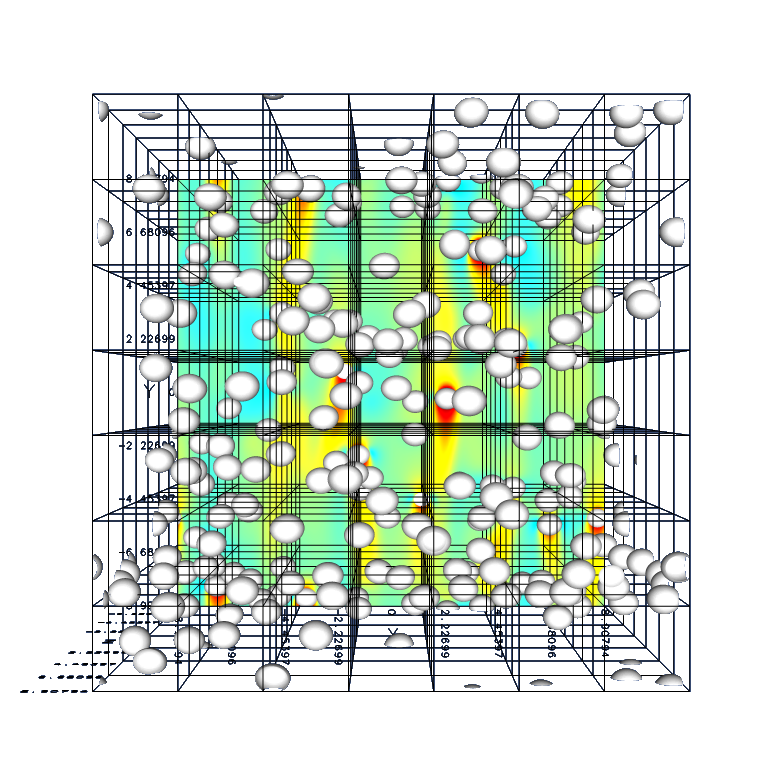
\includegraphics[width = 0.8 \textwidth]{image/PHI_01_Ga_75.png}
    \caption{Snapshot of a simulation at $T_g = 300$ for $\phi = 0.1$, $Ga = 75$ $\mu_r = 0.1$ and $N_b = 125$. In white : the interfaces, The background color map correspond to the pressure field. The grid represents the different core.}
    \label{fig:pic_sim}
\end{figure*}
As a consequence of the mono-disperse assumption it is evident that the mass balance and number density balance are similar. 
However, the surface balance (\ref{eq:A_avg_p}) remains relevant as the surface of all particles is not constant since it is a function of the deformation. 
However, as it will be shown in the low \textit{Bond} numbers limit the droplets remain spherical allowing us o discard this equation too. 
Therefore, In this context we be interested in the momentum balance's (\ref{eq:classic_hybrid_momentum_p} and \ref{eq:classic_hybrid_momentum_c}) closures. 
Neglecting the mass transfer terms and considering the mass as a constant yields the following particular and continuous averaged momentum equations, 
\begin{multline}
    \rho_c\pddt (\phi_c\cavg{\textbf{u}}) 
    + \rho_c\grad \cdot ( \phi_c \cavg{\textbf{u}}\cavg{\textbf{u}})
    = \pavg{\int_{S_\alpha} \textbf{T}_c  \cdot \textbf{n}_c d S}
    +\phi_c\cavg{\textbf{b}}\\
    + \grad\cdot\left[
    \phi_c \cavg{\textbf{T}}
    - \pavg{\int_{S_\alpha} \textbf{r} \textbf{T}_c  \cdot \textbf{n}_c dS}
    - \rho \cavg{\textbf{u}'\textbf{u}'}
    \right],
    \label{eq:homo_momentum_c}
\end{multline}
\begin{multline}
    \pddt   \left(\pavg{\textbf{u}_\alpha}\right)
    + \grad \cdot \left(\pavg{\textbf{u}_\alpha}\pnavg{\textbf{u}_\alpha}\right)
    = \frac{n}{m_\alpha}\pnavg{\int_{V_\alpha} \textbf{b} dV}\\
    + \frac{n}{m_\alpha}\pnavg{\int_{S_\alpha} \textbf{T}_c  \cdot \textbf{n}_c dS}
    - \grad \cdot \left(\pavg{\textbf{u}_\alpha' \textbf{u}_\alpha'}\right). 
    \label{eq:homo_momentum_p}
\end{multline}
From these simplified equations we can start to complete the closure problem.

Since all simulations reach as quasi static regime we can stipulate that the averaged velocities vector are constants and vertical. 
Therefore, all along this chapter we note the drift velocity such as $U = \pnavg{\textbf{u}} - \cavg{\textbf{u}}$. 
Besides, in this chapter we fix the following dimensionless parameters to $\rho_r =1.11 $, $\mu_r =0.1$, $Bo =1$ and $N_b = 125$. 
As a consequence of the small \textit{Bond} number in presence, the droplets are nearly spherical. 
A picture of a typical simulation is shown \ref{fig:pic_sim}